\documentclass[border=2pt]{standalone}
\usepackage{fontspec}
\setmainfont{TeX Gyre Pagella}
\usepackage{pgfplots}
\pgfplotsset{compat=1.18}
\usepackage{amsmath}
\begin{document}
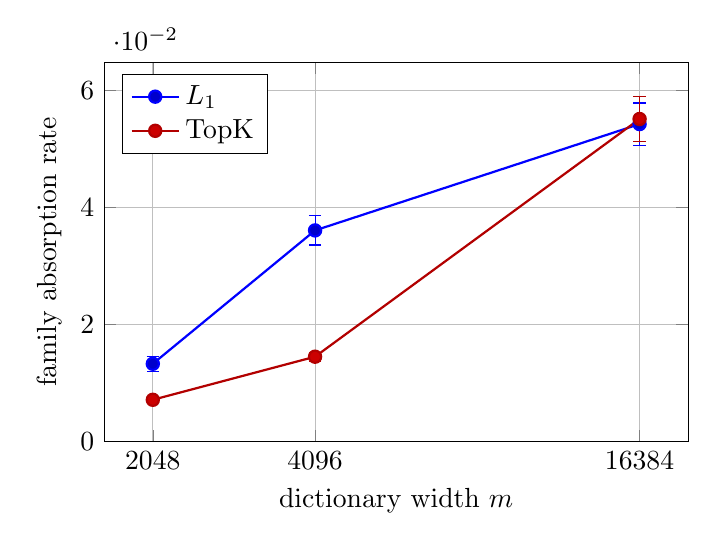
\begin{tikzpicture}
\begin{axis}[width=9cm,height=6.4cm,xmode=log,log basis x=2,
  xlabel={dictionary width $m$},ylabel={family absorption rate},
  xtick={2048,4096,16384},xticklabels={2048,4096,16384},
  legend pos=north west,legend cell align=left,grid=major,
  ymin=0,every axis plot/.append style={thick,mark size=2.2pt}]
\addplot+[color=blue,mark=*,error bars/.cd,y dir=both,y explicit] coordinates {(2048,0.01328) +- (0,0.00131) (4096,0.03606) +- (0,0.00249) (16384,0.05422) +- (0,0.00360)};
\addlegendentry{$L_1$}
\addplot+[color=red!70!black,mark=*,error bars/.cd,y dir=both,y explicit] coordinates {(2048,0.00713) +- (0,0.00052) (4096,0.01449) +- (0,0.00078) (16384,0.05509) +- (0,0.00382)};
\addlegendentry{TopK}
\end{axis}
\end{tikzpicture}
\end{document}
